\documentclass{beamer}
\usepackage{beamerthemesplit}
\usepackage{wrapfig}
\usetheme{SPbGU}
\usepackage{pdfpages}
\usepackage{amsmath}
\usepackage{cmap} 
\usepackage[T2A]{fontenc} 
\usepackage[utf8]{inputenc}
\usepackage[english,russian]{babel}
\usepackage{indentfirst}
\usepackage{amsmath}
\usepackage{tikz}
\usepackage{multirow}
\usepackage[noend]{algpseudocode}
\usepackage{algorithm}
\usepackage{algorithmicx}
\usetikzlibrary{shapes,arrows}
\usepackage{fancyvrb}
\newtheorem{rutheorem}{Теорема}
\newtheorem{ruproof}{Доказательство}
\newtheorem{rudefinition}{Определение}
\newtheorem{rulemma}{Лемма}
\beamertemplatenavigationsymbolsempty

\title[]{Разработка системы предсказания вторичной структуры РНК с использованием синтаксического анализа и искусственных нейронных сетей}
%\subtitle[]{Опциональный подзаголовок}
% То, что в квадратных скобках, отображается в левом нижнем углу. 
\institute[СПбГУ]{
Санкт-Петербургский государственный университет \\
Кафедра системного программирования }

% То, что в квадратных скобках, отображается в левом нижнем углу.
\author[Кутленков Дмитрий]{Кутленков Дмитрий Александрович, 371 группа(17.Б11-мм) \\
  % У научного руководителя должна быть указана научная степень
  \and  
    {\bfseries Научный руководитель:} к.ф.-м.н., доцент Григорьев С.В. \\ 
  % Для курсовой не обязателен. Должна быть указана должность или ученая степень
%  \and
%    {\bfseries Рецензент:} программист ООО ``Рога и копыта'' И.И. Иванов
}

\date{2 мая 2020г.}

\definecolor{orange}{RGB}{179,36,31}

\begin{document}
{
% Лого университета или организации, отображается в шапке титульного листа
\begin{frame}
  \begin{center}
  {
\includegraphics[width=1.5cm]{pictures/SPbGU_Logo.png}}
  \end{center}
  \titlepage
\end{frame}
}

\begin{frame}[fragile]
  \transwipe[direction=90]
  \frametitle{Введение}
  
%    \item Краткий обзор тематики работы (как вариант — устно, пока показывается титульный слайд)
%    \item Не нужно определять общеизвестные понятия
%    \item Применимость/полезность данной работы, обоснование выбора именно этой темы 
%    \item Если тема похожа на темы других работ (в том числе прошлых лет), надо явно описать разницу
\begin{tabular}{p{5cm} p{7cm}}
	\begin{itemize}
		\item РНК - биологическая последовательность
		\item Ее первичная структура - последовательность нуклеотидов, которые задаются алфавитом из 4 букв
		\item Вторичная структура - то, как нуклеотиды образуют связи 
		\item Псевдоузел - новая петля начинается до конца предыдущей
  \end{itemize} &
%{\includegraphics[width=5cm]{../DNA_RNA_structure_(full).png}}
\multirow{-1.5}*{\!\includegraphics[width=4.5cm]{../pics/DNA_RNA_structure_(full).png}}
\end{tabular}

\end{frame}
            
\begin{frame}
  \transwipe[direction=90]
  \frametitle{Существующие решения}
  \begin{itemize}
  	\item Методы сравнительного анализа
    \item Метод минимальной свободной энергии (MFE) - \textit{RNAfold}, \textit{CentroidFold}, \textit{HotKnots}, \textit{IPknot}
    \item Иерархическая свертка - \textit{HFold}, \textit{Iterative HFold}
    \item Исследования с использованием машинного обучения
   
  \end{itemize}\medskip
   Не существует оптимального метода.

\end{frame}

% Обязательный слайд: четкая формулировка цели данной работы и постановка задачи
% Описание выносимых на защиту результатов, процесса или особенностей их достижения и т.д.
\begin{frame}
  \transwipe[direction=90]
  \frametitle{Постановка задачи}
  \textbf{Целью} данной работы является разработка системы, способной с достаточной степенью точности предсказывать вторичную структуру РНК 
  
  \textbf{Задачи}:
  \begin{itemize}
    \item Изучить предметную область
    \item Проанализировать существующие решения
    \item Спроектировать систему на основе формальных грамматик и нейронных сетей
    \item Собрать и обработать данные для обучения нейронной сети
    \item Создать систему для подготовки данных
    \item Обработать результат нейронной сети для получения биологически возможного результата
    \item Собрать составные части в единую систему, с которой будет удобно работать целевой аудитории, то есть биологам и биоинформатикам
  \end{itemize}
\end{frame}
            
%\begin{frame}[fragile]
%\transwipe[direction=90]
%\frametitle{Иллюстративные возможности: таблицы, картинки, код}
%% Задается ширина столбцов
%\begin{tabular}{p{5cm} p{7cm}}
%% Фрагмент кода
%\begin{minipage}{3in}
%  \begin{Verbatim}[commandchars=\\\{\}]
%
%\textcolor{blue}{string} res = \textcolor{orange}{""};
%\textcolor{blue}{for}(i = 0; i < l; i++) \{
%    res = \textcolor{orange}{"()"} + res;
%\}   
%
%  \end{Verbatim}
%\end{minipage}
%&
%Результат (SPPF):
%\\
%Аппроксимация: 
%&
%% Картинка
%\multirow{-2}*{\!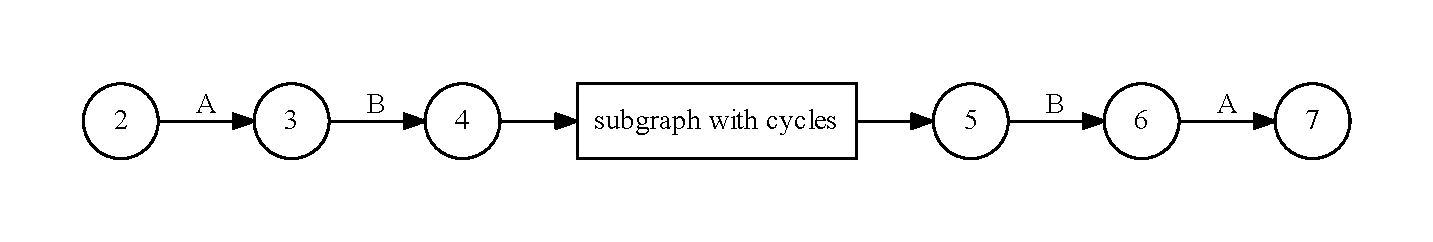
\includegraphics[width=6.8cm]{pictures/out3.pdf}}
%\\
%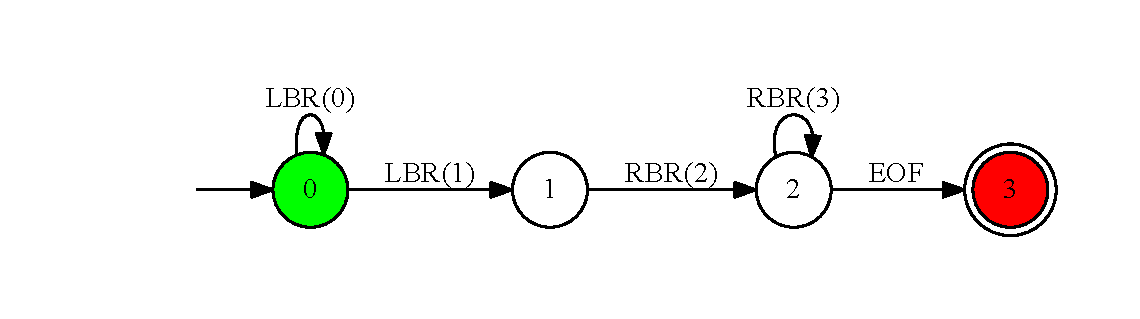
\includegraphics[width=3cm]{pictures/in3.pdf}
%&
%\\      
%Грамматика: &
%\\
%\vspace{-20pt}
%% Можно формулы писать
%$$
%\begin{array}{crcl}
%&start &::=& s \\
%&s & ::= & \mbox{\texttt{LBR }} s \mbox{\texttt{ RBR }} s\\
%&s & ::= &\epsilon
%\end{array}
%$$
%& 
%\end{tabular}
%\end{frame}

\begin{frame}[fragile]
\transwipe[direction=90]
\frametitle{Архитектура системы подготовки данных}
\begin{tabular}{p{5cm} p{7cm}}
	\begin{itemize}
		\item Парсер - распознает места возможных связей
		\item Нейросеть - учится очищать результат работы парсера
		\item Представление данных в виде изображений
	\end{itemize} &
	\multirow{-3}*{\!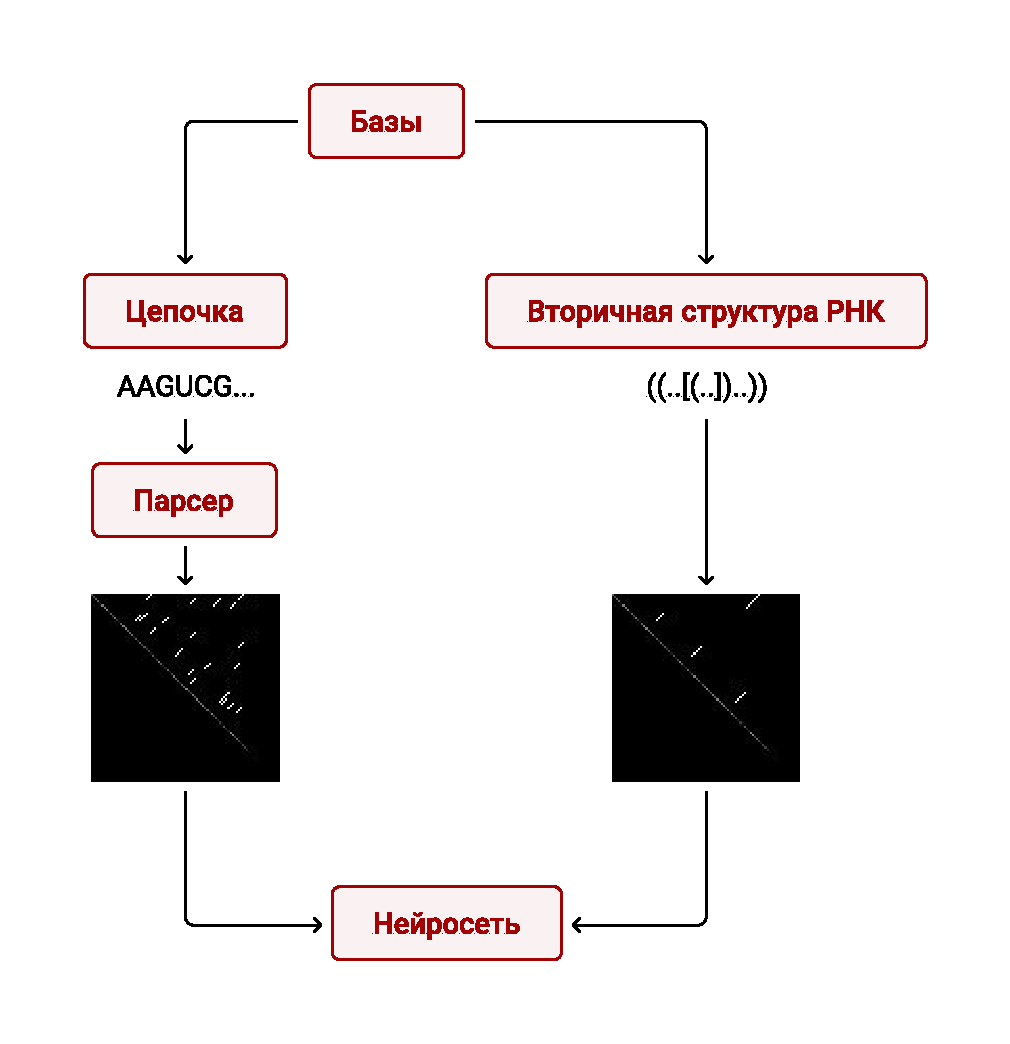
\includegraphics[width=7cm]{pictures/diag2.pdf}}\\
	\multirow{-1.75}*{\!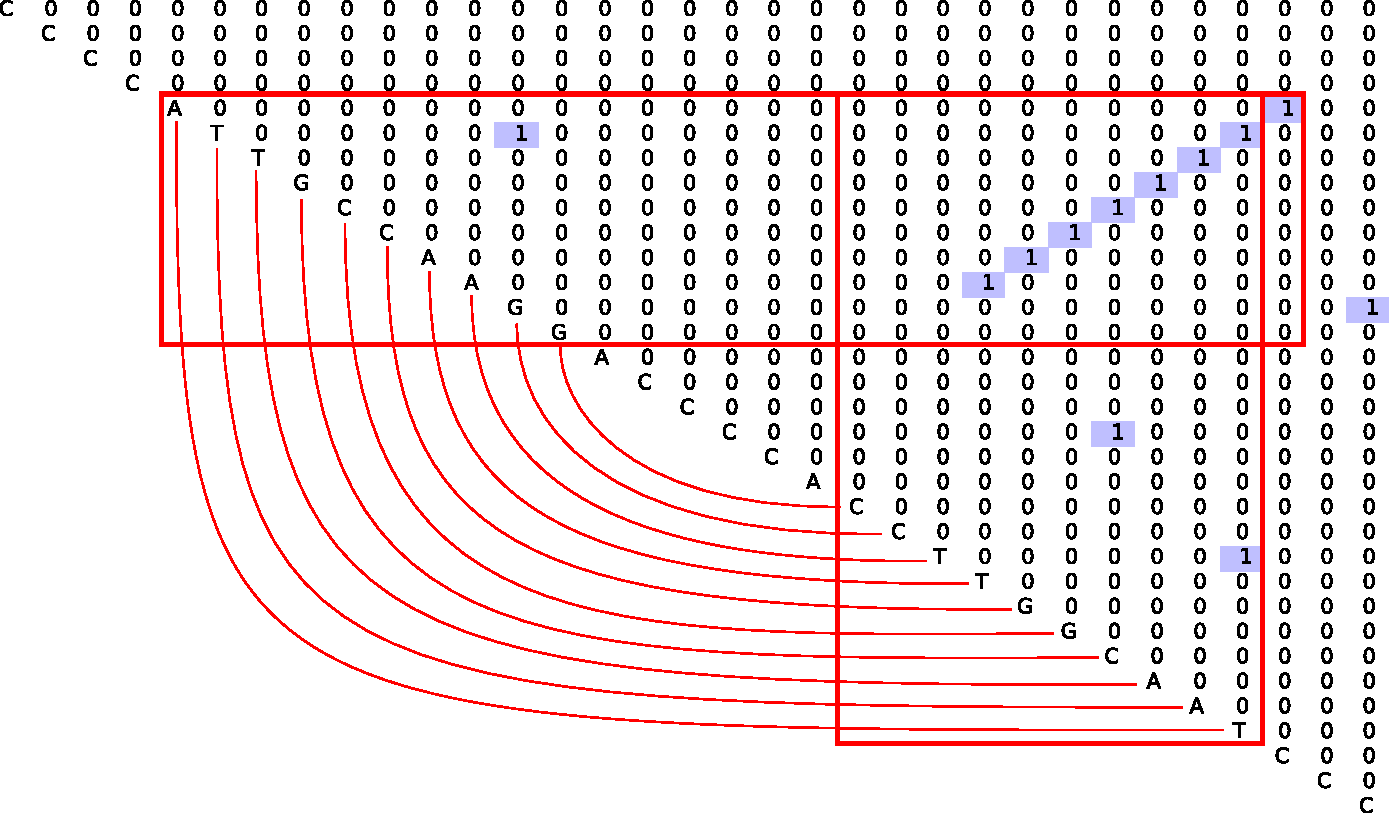
\includegraphics[width=4.5cm]{../pics/4.pdf}}
\end{tabular}

\end{frame}
\begin{frame}[fragile]
\transwipe[direction=90]
\frametitle{Архитектура конечной системы}
\begin{tabular}{p{5cm} p{7cm}}
	\begin{itemize}
		\item Клиент-серверное приложение
		\item Пользователь может видеть промежуточные этапы работы системы
		\item Результат выраванивается, чтобы соответствовать биологическим законам
		
		
	\end{itemize} &
	%{\includegraphics[width=5cm]{../DNA_RNA_structure_(full).png}}
	\multirow{-2}*{\!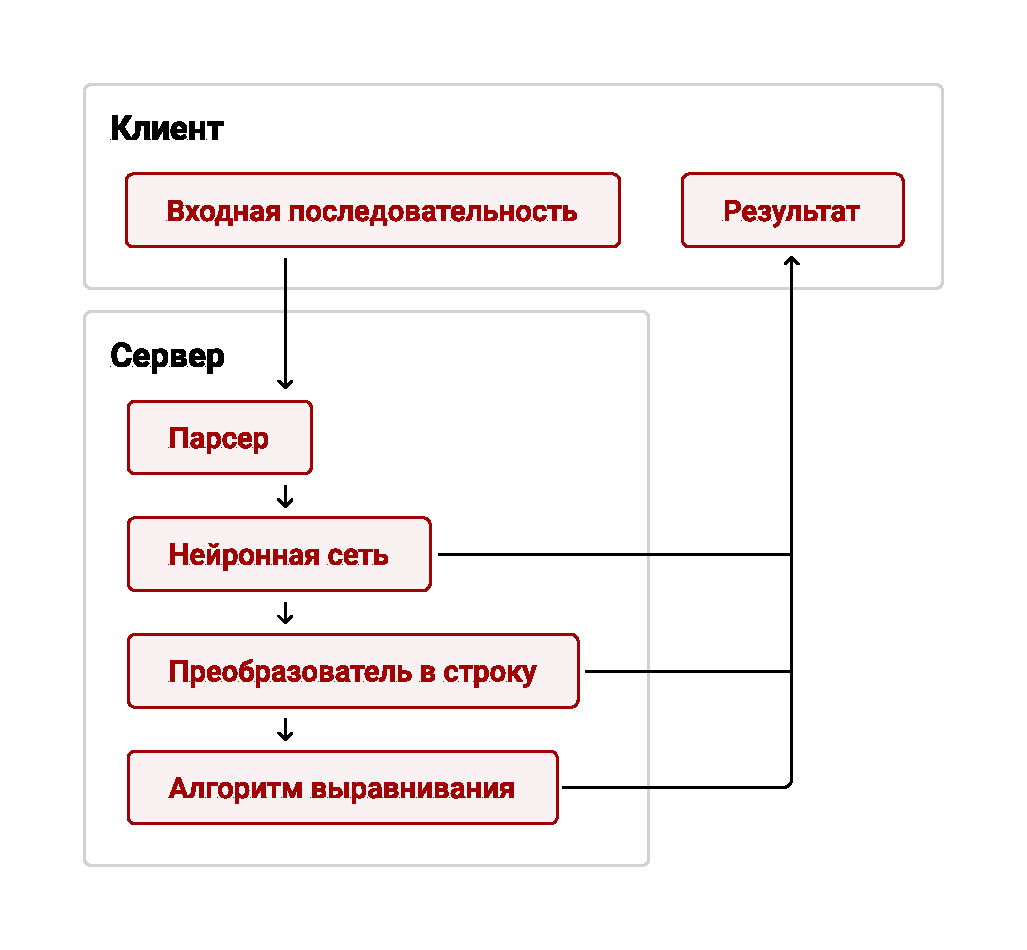
\includegraphics[width=7cm]{pictures/diag1.pdf}}
\end{tabular} \\ \bigskip 
Система доступна по адресу \url{http://www.secondarystructure.tk/}

\end{frame}

\begin{frame}
\transwipe[direction=90]
\frametitle{Используемые технологии}
\begin{itemize}
	\item Связь через \textit{REST API}
	\item Сервер - \textit{Python3}, \textit{Flask}, \textit{Waitress}, \textit{Biopython}
	\item Клиент - \textit{Bulma.io}, \textit{Vue.js}, \textit{axios}
	
\end{itemize}\medskip

\end{frame}
	


\begin{frame}
  \transwipe[direction=90]
  \frametitle{Результаты}
  \begin{itemize}
    \item Изучена предметная область
    \item Проведен анализ уже существующих решений
    \item Разработана архитектура системы
    \item Собраны, проанализированы и обработаны данные из нескольких источников - \textit{RNA STRAND}, \textit{Pseudobase++}, \textit{RNACentral}
    \item Создана система подготовки данных
    \item Разработан алгоритм перевода полученных последовательностей в биологически возможные
    \item Разработана система предсказания вторичной структуры РНК последовательностей
    \item Создано клиент-серверное приложение, предоставляющее доступ к системе
  \end{itemize}
\end{frame}

\end{document}
